% Arquivo LaTeX de exemplo de dissertação/tese a ser apresentada à CPG do IME-USP
%
% Criação: Jesús P. Mena-Chalco
% Revisão: Fabio Kon e Paulo Feofiloff
% Adaptação para UTF8, biblatex e outras melhorias: Nelson Lago
%
% Except where otherwise indicated, these files are distributed under
% the MIT Licence. The example text, which includes the tutorial and
% examples as well as the explanatory comments in the source, are
% available under the Creative Commons Attribution International
% Licence, v4.0 (CC-BY 4.0) - https://creativecommons.org/licenses/by/4.0/


%%%%%%%%%%%%%%%%%%%%%%%%%%%%%%%%%%%%%%%%%%%%%%%%%%%%%%%%%%%%%%%%%%%%%%%%%%%%%%%%
%%%%%%%%%%%%%%%%%%%%%%%%%%%%%%% PREÂMBULO LaTeX %%%%%%%%%%%%%%%%%%%%%%%%%%%%%%%%
%%%%%%%%%%%%%%%%%%%%%%%%%%%%%%%%%%%%%%%%%%%%%%%%%%%%%%%%%%%%%%%%%%%%%%%%%%%%%%%%

% A opção twoside (frente-e-verso) significa que a aparência das páginas pares
% e ímpares pode ser diferente. Por exemplo, as margens podem ser diferentes ou
% os números de página podem aparecer à direita ou à esquerda alternadamente.
% Mas nada impede que você crie um documento "só frente" e, ao imprimir, faça
% a impressão frente-e-verso.
%
% Aqui também definimos a língua padrão do documento (a última da lista) e
% línguas adicionais. Para teses do IME, no mínimo português e inglês são
% obrigatórios, porque independentemente da língua principal do texto é
% preciso fornecer o resumo nessas duas línguas. LaTeX aceita alguns nomes
% diferentes para a língua portuguesa; dentre as opções, prefira sempre
% "brazilian" para português brasileiro e "portuguese" para português europeu.
%\documentclass[a4paper,12pt,twoside,brazilian,english]{book}
\documentclass[a4paper,12pt,twoside,english,brazilian]{book}

% O preâmbulo de um documento LaTeX pode ser razoavelmente longo. Neste
% modelo, optamos por reduzi-lo, colocando praticamente tudo do preâmbulo
% nas packages "imegoodies" e "imelooks".
%
% imegoodies carrega diversas packages muito úteis e populares (algumas
% são praticamente obrigatórias, como amsmath, babel, array etc.). É
% uma boa ideia usá-la com outros documentos também. Ela inclui vários
% comentários explicativos e dicas de uso; não tenha medo de alterá-la
% conforme a necessidade.
%
% imelooks carrega algumas packages e configurações que definem a
% aparência do documento; você também pode querer usá-la (ou partes
% dela) com outros documentos para obter as mesmas fontes, margens
% etc. Tal como "imegoodies", pode valer a pena ler os comentários
% e fazer modificações nessa package. Com a opção "thesis", imelooks
% também define os comandos para capa, folha de rosto etc.
\usepackage{imegoodies}
\usepackage[thesis]{imelooks}

%\nocolorlinks % para impressão em P&B

% Diretórios onde estão as figuras; com isso, não é necessário (mas
% é permitido) colocar o caminho completo em \includegraphics. Note
% que a extensão nunca é necessária (mas é permitida), ou seja, o
% resultado é o mesmo com "\includegraphics{figuras/foto.jpeg}",
% "\includegraphics{foto.jpeg}", "\includegraphics{figuras/foto}"
% ou "\includegraphics{foto}".
\graphicspath{{figuras/},{fig/},{logos/},{img/},{images/},{imagens/}}

% Comandos rápidos para mudar de língua:
% \en -> muda para o inglês
% \br -> muda para o português
% \texten{blah} -> o texto "blah" é em inglês
% \textbr{blah} -> o texto "blah" é em português
\babeltags{br = brazilian, en = english}


%%%%%%%%%%%%%%%%%%%%%%%%%%%%%%%%%%%%%%%%%%%%%%%%%%%%%%%%%%%%%%%%%%%%%%%%%%%%%%%%
%%%%%%%%%%%%%%%%%%%%%%%%%%%%%%%%%% METADADOS %%%%%%%%%%%%%%%%%%%%%%%%%%%%%%%%%%%
%%%%%%%%%%%%%%%%%%%%%%%%%%%%%%%%%%%%%%%%%%%%%%%%%%%%%%%%%%%%%%%%%%%%%%%%%%%%%%%%

% O arquivo com os dados bibliográficos para biblatex; você pode usar
% este comando mais de uma vez para acrescentar múltiplos arquivos
\addbibresource{bibliografia.bib}

% Este comando permite acrescentar itens à lista de referências sem incluir
% uma referência de fato no texto (pode ser usado em qualquer lugar do texto)
%\nocite{bronevetsky02,schmidt03:MSc, FSF:GNU-GPL, CORBA:spec, MenaChalco08}
% Com este comando, todos os itens do arquivo .bib são incluídos na lista
% de referências
%\nocite{*}

% É possível definir como determinadas palavras podem (ou não) ser
% hifenizadas; no entanto, a hifenização automática geralmente funciona bem
\babelhyphenation{documentclass latexmk soft-ware clsguide} % todas as línguas
\babelhyphenation[brazilian]{Fu-la-no}
\babelhyphenation[english]{what-ever}

% Estes comandos definem o título e autoria do trabalho e devem sempre ser
% definidos, pois além de serem utilizados para criar a capa, também são
% armazenados nos metadados do PDF. O subtítulo é opcional.
\title{Grafos: legal demais!}
\translatedtitle{Graphs: so cool!}

\author{Marcelo Machado Lage}

\def\prof{Prof\kern.02em.\kern-.07em\kern.07em}
\def\dr{Dr\kern-.04em.\kern-.11em\kern.07em}

% Para TCCs, este comando define o supervisor
\orientador{\prof{} \dr{} Guilherme Oliveira Mota}


% A página de rosto da versão para depósito (ou seja, a versão final
% antes da defesa) deve ser diferente da página de rosto da versão
% definitiva (ou seja, a versão final após a incorporação das sugestões
% da banca).
\tipotese{
  %mestrado,
  %doutorado,
  tcc,
  %definitiva, % É a versão para defesa ou a versão definitiva?
  %quali, % É qualificação?
  programa={Ciência da Computação},
}

\defesa{
  local={São Paulo},
  data=2025-12-31, % YYYY-MM-DD
}

% Se não houve bolsa, remova
%
% Norma sobre agradecimento por auxílios da FAPESP:
% https://fapesp.br/11789/referencia-ao-apoio-da-fapesp-em-todas-as-formas-de-divulgacao
%
% Norma sobre agradecimento por auxílios da CAPES (Portaria 206,
% de 4 de Setembro de 2018):
% https://www.in.gov.br/materia/-/asset_publisher/Kujrw0TZC2Mb/content/id/39729251/do1-2018-09-05-portaria-n-206-de-4-de-setembro-de-2018-39729135
%
%\apoio{O presente trabalho foi realizado com apoio da Coordenação
%      de Aperfeiçoamento\\ de Pessoal de Nível Superior -- Brasil
%      (CAPES) -- Código de Financiamento 001} % o código é sempre 001
%
%\apoio{This study was financed in part by the Coordenação de
%      Aperfeiçoamento\\ de Pessoal de Nível Superior -- Brasil
%      (CAPES) -- Finance Code 001} % o código é sempre 001
%
%\apoio{Durante o desenvolvimento deste trabalho, o autor recebeu\\
%      auxílio financeiro da FAPESP -- processo nº aaaa/nnnnn-d}
%
%\apoio{During the development if this work, the author received\\
%      financial support from FAPESP -- grant \#aaaa/nnnnn-d}
\apoio{Durante o desenvolvimento deste trabalho o autor
       recebeu auxílio financeiro da FAPESP}

% A licença do seu trabalho. Use CC-BY, CC-BY-NC, CC-BY-ND, CC-BY-SA,
% CC-BY-NC-SA ou CC-BY-NC-ND para escolher a licença Creative Commons
% correspondente (o sistema insere automaticamente o texto da licença).
% Se quiser estabelecer regras diferentes para o uso de seu trabalho,
% converse com seu orientador e coloque o texto da licença aqui, mas
% observe que apenas TCCs sob alguma licença Creative Commons serão
% acrescentados ao BDTA. Se você tem alguma intenção de publicar o
% trabalho comercialmente no futuro, sugerimos a licença CC-BY-NC-ND.
%
%\direitos{CC-BY-NC-ND}
%
%\direitos{Autorizo a reprodução e divulgação total ou parcial deste
%          trabalho, por qualquer meio convencional ou eletrônico,
%          para fins de estudo e pesquisa, desde que citada a fonte.}
%
%\direitos{I authorize the complete or partial reproduction and disclosure
%          of this work by any conventional or electronic means for study
%          and research purposes, provided that the source is acknowledged.}
%
\direitos{CC-BY}

% Para gerar a ficha catalográfica, acesse https://fc.ime.usp.br/,
% preencha o formulário e escolha a opção "Gerar Código LaTeX".
% Basta copiar e colar o resultado aqui.
\fichacatalografica{}


%%%%%%%%%%%%%%%%%%%%%%%%%%%%%%%%%%%%%%%%%%%%%%%%%%%%%%%%%%%%%%%%%%%%%%%%%%%%%%%%
%%%%%%%%%%%%%%%%%%%%%%% AQUI COMEÇA O CONTEÚDO DE FATO %%%%%%%%%%%%%%%%%%%%%%%%%
%%%%%%%%%%%%%%%%%%%%%%%%%%%%%%%%%%%%%%%%%%%%%%%%%%%%%%%%%%%%%%%%%%%%%%%%%%%%%%%%

\begin{document}

%%%%%%%%%%%%%%%%%%%%%%%%%%% CAPA E PÁGINAS INICIAIS %%%%%%%%%%%%%%%%%%%%%%%%%%%%

% Aqui começa o conteúdo inicial que aparece antes do capítulo 1, ou seja,
% página de rosto, resumo, sumário etc. O comando frontmatter faz números
% de página aparecem em algarismos romanos ao invés de arábicos e
% desabilita a contagem de capítulos.
\frontmatter

\pagestyle{plain}

\onehalfspacing % Espaçamento 1,5 na capa e páginas iniciais

\maketitle % capa e folha de rosto

%%%%%%%%%%%%%%%% DEDICATÓRIA, AGRADECIMENTOS, RESUMO/ABSTRACT %%%%%%%%%%%%%%%%%%

%\begin{dedicatoria}
%Esta seção é opcional e fica numa página separada; ela pode ser usada para
%uma dedicatória ou epígrafe.
%\end{dedicatoria}

% Reinicia o contador de páginas (a próxima página recebe o número "i") para
% que a página da dedicatória não seja contada.
\pagenumbering{roman}


%!TeX root=../tese.tex
%("dica" para o editor de texto: este arquivo é parte de um documento maior)
% para saber mais: https://tex.stackexchange.com/q/78101

% As palavras-chave são obrigatórias, em português e em inglês, e devem ser
% definidas antes do resumo/abstract. Acrescente quantas forem necessárias.
\palavraschave{Palavra-chave1, Palavra-chave2, Palavra-chave3}

\keywords{Keyword1,Keyword2,Keyword3}

% O resumo é obrigatório, em português e inglês. Estes comandos também
% geram automaticamente a referência para o próprio documento, conforme
% as normas sugeridas da USP.
\resumo{
Elemento obrigatório, constituído de uma sequência de frases concisas e
objetivas, em forma de texto. Deve apresentar os objetivos, métodos empregados,
resultados e conclusões. O resumo deve ser redigido em parágrafo único, conter
no máximo 500 palavras e ser seguido dos termos representativos do conteúdo do
trabalho (palavras-chave). Deve ser precedido da referência do documento.
Texto texto texto texto texto texto texto texto texto texto texto texto texto
texto texto texto texto texto texto texto texto texto texto texto texto texto
texto texto texto texto texto texto texto texto texto texto texto texto texto
texto texto texto texto texto texto texto texto texto texto texto texto texto
texto texto texto texto texto texto texto texto texto texto texto texto texto
texto texto texto texto texto texto texto texto.
Texto texto texto texto texto texto texto texto texto texto texto texto texto
texto texto texto texto texto texto texto texto texto texto texto texto texto
texto texto texto texto texto texto texto texto texto texto texto texto texto
texto texto texto texto texto texto texto texto texto texto texto texto texto
texto texto.
}

\abstract{
Elemento obrigatório, elaborado com as mesmas características do resumo em
língua portuguesa. De acordo com o Regimento da Pós-Graduação da USP (Artigo
99), deve ser redigido em inglês para fins de divulgação. É uma boa ideia usar
o sítio \url{www.grammarly.com} na preparação de textos em inglês.
Text text text text text text text text text text text text text text text text
text text text text text text text text text text text text text text text text
text text text text text text text text text text text text text text text text
text text text text text text text text text text text text.
Text text text text text text text text text text text text text text text text
text text text text text text text text text text text text text text text text
text text text.
}



%%%%%%%%%%%%%%%%%%%%%%%%%%% LISTAS DE FIGURAS ETC. %%%%%%%%%%%%%%%%%%%%%%%%%%%%%

% Como as listas que se seguem podem não incluir uma quebra de página
% obrigatória, inserimos uma quebra manualmente aqui.
%\cleardoublepage

% Todas as listas são opcionais; Usando "\chapter*" elas não são incluídas
% no sumário. As listas geradas automaticamente também não são incluídas por
% conta das opções "notlot" e "notlof" que usamos para a package tocbibind.

% Normalmente, "\chapter*" faz o novo capítulo iniciar em uma nova página, e as
% listas geradas automaticamente também por padrão ficam em páginas separadas.
% Como cada uma destas listas é muito curta, não faz muito sentido fazer isso
% aqui, então usamos este comando para desabilitar essas quebras de página.
% Se você preferir, comente as linhas com esse comando e des-comente as linhas
% sem ele para criar as listas em páginas separadas. Observe que você também
% pode inserir quebras de página manualmente (com \clearpage, veja o exemplo
% mais abaixo).
%\newcommand\disablenewpage[1]{{\let\clearpage\par\let\cleardoublepage\par #1}}

% Nestas listas, é melhor usar "raggedbottom" (veja basics.tex). Colocamos
% a opção correspondente e as listas dentro de um grupo para ativar
% raggedbottom apenas temporariamente.
%\bgroup
%\raggedbottom

%%%%% Listas criadas manualmente

%\chapter*{Lista de abreviaturas}
%\disablenewpage{\chapter*{Lista de abreviaturas}}

%\begin{tabular}{rl}
%   CFT & Transformada contínua de Fourier (\emph{Continuous Fourier Transform})\\
%   DFT & Transformada discreta de Fourier (\emph{Discrete Fourier Transform})\\
%  EIIP & Potencial de interação elétron-íon (\emph{Electron-Ion Interaction Potentials})\\
%  STFT & Transformada de Fourier de tempo reduzido (\emph{Short-Time Fourier Transform})\\
%  ABNT & Associação Brasileira de Normas Técnicas\\
%   URL & Localizador Uniforme de Recursos (\emph{Uniform Resource Locator})\\
%   IME & Instituto de Matemática e Estatística\\
%   USP & Universidade de São Paulo
%\end{tabular}

%\chapter*{Lista de símbolos}
%\disablenewpage{\chapter*{Lista de símbolos}}
%
%\begin{tabular}{rl}
%  $\omega$ & Frequência angular\\
%    $\psi$ & Função de análise \emph{wavelet}\\
%    $\Psi$ & Transformada de Fourier de $\psi$\\
%\end{tabular}

% Quebra de página manual
%\clearpage

%%%%% Listas criadas automaticamente

% Você pode escolher se quer ou não permitir a quebra de página
%\listoffigures
%\disablenewpage{\listoffigures}

% Você pode escolher se quer ou não permitir a quebra de página
%\listoftables
%\disablenewpage{\listoftables}

% Esta lista é criada "automaticamente" pela package float quando
% definimos o novo tipo de float "program" (em utils.tex)
% Você pode escolher se quer ou não permitir a quebra de página
%\listof{program}{\programlistname}
%\disablenewpage{\listof{program}{\programlistname}}

% Sumário (obrigatório)
\tableofcontents

%\egroup % Final de "raggedbottom"

% Referências indiretas ("x", veja "y") para o índice remissivo (opcionais,
% pois o índice é opcional). É comum colocar esses itens no final do documento,
% junto com o comando \printindex, mas em alguns casos isso torna necessário
% executar texindy (ou makeindex) mais de uma vez, então colocar aqui é melhor.
\index{Inglês|see{Língua estrangeira}}
\index{Figuras|see{Floats}}
\index{Tabelas|see{Floats}}
\index{Código-fonte|see{Floats}}
\index{Subcaptions|see{Subfiguras}}
\index{Sublegendas|see{Subfiguras}}
\index{Equações|see{Modo matemático}}
\index{Fórmulas|see{Modo matemático}}
\index{Rodapé, notas|see{Notas de rodapé}}
\index{Captions|see{Legendas}}
\index{Versão original|see{Tese/Dissertação, versões}}
\index{Versão corrigida|see{Tese/Dissertação, versões}}
\index{Palavras estrangeiras|see{Língua estrangeira}}
\index{Floats!Algoritmo|see{Floats, ordem}}


%%%%%%%%%%%%%%%%%%%%%%%%%%%%%%%% CAPÍTULOS %%%%%%%%%%%%%%%%%%%%%%%%%%%%%%%%%%%%%

% Aqui vai o conteúdo principal do trabalho, ou seja, os capítulos que compõem
% a dissertação/tese. O comando mainmatter reinicia a contagem de páginas,
% modifica a numeração para números arábicos e ativa a contagem de capítulos.
\mainmatter

\pagestyle{mainmatter}

% Espaçamento simples
\singlespacing

% A introdução não tem número de capítulo, então os cabeçalhos também não
\pagestyle{unnumberedchapter}
\pagestyle{mainmatter}



\chapter{Resultados clássicos}
\label{cap:classicos}

\theoremstyle{plain}
\newtheorem{theorem}{Teorema}

\theoremstyle{plain}
\newtheorem{conjecture}{Conjectura}

\theoremstyle{plain}
\newtheorem{claim}{Afirmação}

\theoremstyle{plain}
\newtheorem{corollary}{Corolário}

\theoremstyle{definition}
\newtheorem{definition}{Definição}

Seja $G$ um grafo. Defininimos $D(G)$ como o menor tamanho de um $F \subseteq E(G)$ tal que $G-F$ é bipartido.

\begin{theorem}[Mantel]
  Seja $G$ um grafo livre de triângulos com $n$ vértices.
  Então $e(G) \leq \left\lceil\frac{n^2}{4}\right\rceil$.
  Além disso, se vale a igualdade então $G$ é bipartido completo.
\end{theorem}

\begin{theorem}[Estabilidade] \label{thm:estabilidade}
  Seja $m$ um inteiro positivo e seja $G$ um grafo livre de triângulos com $n$ vértices e $\frac{n^2}{4}-m$ arestas.
  Então $D(G) \leq m$.
\end{theorem}

\begin{conjecture}[Erd\H os] \label{conj:make-bipartite}
  Seja $G$ um grafo livre de triângulos com $n$ vértices.
  Então $G$ pode ser tornado bipartido pela remoção de no máximo $\frac{n^2}{25}$ arestas.
\end{conjecture}

Observe que o Teorema \ref{thm:estabilidade} prova a Conjetura para grafos suficientemente densos (com pelo menos $\frac{n^2}{4} - \frac{n^2}{25}$ arestas).

\begin{definition}
  Sejam $G$ um grafo e $H$ um blow-up de $G$, com $\phi \colon V(H) \to V(G)$ sendo um homomorfismo que define esse blow-up.
  Dizemos que um $S \subseteq E(H)$ é \textit{canônico com relação a $\phi$} se para quaisquer $e,f \in E(H)$ com
  $\phi(e)=\phi(f)$ vale que $e \in S \iff f \in S$.
  Em outras palavras, entre cada par de classes de $H$ escolhemos ou todas as arestas entre essas classes ou não escolhemos nenhuma dessas arestas.
  
  Se $\phi$ for claro do contexto, iremos omitir e dizer apenas que o conjunto de arestas do blow-up é canônico.
\end{definition}

\begin{theorem}[Simetrização]
  Seja $G$ um grafo livre de triângulos e seja $H$ um blow-up de $G$.
  Então existe $F \subseteq E(H)$ canônico com $|F|=D(H)$ e tal que $G-F$ é bipartido.
\end{theorem}

\begin{corollary}
  Seja $H$ um blow-up de $C_5$ com $n$ vértices.
  Então \[ D(H) \leq \frac{n^2}{25}. \]
  Em particular, a Conjectura \ref{conj:make-bipartite} (se verdadeira) dá a melhor constante possível.
\end{corollary}

\begin{theorem}
  Seja $G$ um grafo livre de triângulo com $n$ vértices e $m$ arestas.
  Então \[ D(G) \leq m-\frac{m^2}{4n}. \]
\end{theorem}

\begin{corollary} \label{cor:n2/5}
  Para todo $n$ inteiro positivo, a conjectura \ref{conj:make-bipartite}
  é verdadeira para grafos com $n$ vértices e pelo menos $\frac{n^2}{5}$
\end{corollary}



%!TeX root=../tese.tex
\chapter{Álgebras de flag}
\label{cap:flag-algebras}

\newcommand{\emptyflag}{\varnothing}
\newcommand{\isom}{\cong}

% Tikz setup from https://arxiv.org/abs/2103.14179

\newcommand{\vc}[1]{\ensuremath{\vcenter{\hbox{#1}}}}
\tikzset{vtx/.style={inner sep=1.7pt, outer sep=0pt, circle, fill}}
\tikzset{unlabeled_vertex/.style={inner sep=1.7pt, outer sep=0pt, circle, fill, draw=black}}
\tikzset{labeled_vertex/.style={inner sep=2.2pt, outer sep=0pt, rectangle, fill=yellow, draw=black}}
\tikzset{edge_color0/.style={color=black,line width=1.2pt}}
\tikzset{edge_color1/.style={color=red,  line width=1.2pt,opacity=0}}
\tikzset{edge_color2/.style={color=blue, line width=1.2pt,opacity=1}}

\newcommand{\flagone}{ % this is the unlabeled triangel
  \vc{\begin{tikzpicture}[scale=0.5]
    \draw \foreach \x in {0,1,2}{(270+\x*360/3:0.8) coordinate(x\x)};
    \draw[edge_color2] (x0)--(x1)--(x2)--(x0);
    \draw (x0) node[unlabeled_vertex]{};
    \draw (x1) node[unlabeled_vertex]{};
    \draw (x2) node[unlabeled_vertex]{};
  \end{tikzpicture}}
}
\newcommand{\kthree}{\flagone}

\newcommand{\flagtwo}{ % this is the unlabeled edge
  \vc{\begin{tikzpicture}[scale=0.5]
    \draw (225:0.8) coordinate(x0);
    \draw (45:0.8) coordinate(x1);
    \draw[edge_color2] (x0)--(x1);
    \draw (x0) node[unlabeled_vertex]{};
    \draw (x1) node[unlabeled_vertex]{};
  \end{tikzpicture}}
}
\newcommand{\edge}{\flagtwo}

\newcommand{\flagthree}{
  \vc{\begin{tikzpicture}[scale=0.5]
    \draw \foreach \x in {0,1,2}{(270+\x*360/3:0.8) coordinate(x\x)};
    \draw[edge_color2] (x1)--(x2);
    \draw (x0) node[labeled_vertex,label=below:$1$]{};
    \draw (x1) node[unlabeled_vertex]{};
    \draw (x2) node[unlabeled_vertex]{};
  \end{tikzpicture}}
}

\section{Preliminares}

Seja $k \geq 0$ um inteiro.
Um \emph{tipo} de \emph{tamanho} $k$ é um grafo $G$ com $V(G) = [k]$,
i.e. é um grafo com todos os seus vértices rotulados.
O tipo vazio é denotado por $\emptyflag$.

Seja $\sigma$ um tipo de tamanho $k$.
Um \emph{$\sigma$-flag} é um par $(F,\phi)$ em que $\phi \colon [k] \to V(F)$
é um homomorfismo de grafos injetor tal que $F[\phi([k])] \isom \sigma$.


\begin{example}[Mantel]
  Se $\kthree = 0$, então $\edge \leq \frac12$.
\end{example}


\section{Aplicações para a Conjectura \ref{conj:make-bipartite}}

\begin{theorem}
  Se $\kthree = 0$ e $\edge \geq \frac{2}{25}$, então
  $\left\llbracket
  \flagthree
  \right\rrbracket
  \leq \frac{2}{25}$.
\end{theorem}

\begin{corollary}
  Seja $G$ um grafo com $n$ vértices e pelo menos $\frac{n^2}{5}$ arestas.
  Então a Conjectura \ref{conj:make-bipartite} vale para $G$.
\end{corollary}

O ponto é que ter a linguagem de flag algebras facilita obter cotas a partir da ideia de ``cortes locais'' e daí pode automatizar o processo.

\begin{theorem}[Balogh-Clemen-Lidický]
  Seja $G$ um grafo livre de triângulos com $n$ vértices.
  Então, vale que
  \begin{enumerate}
    \item $D(G) \leq \frac{n^2}{23.5}$;
    \item $D(G) \leq \frac{n^2}{25}$ se $e(G) \geq 0.3197 \binom{n}{2}$;
    \item $D(G) \leq \frac{n^2}{25}$ se $e(G) \leq 0.2486 \binom{n}{2}$.
  \end{enumerate}
\end{theorem}

%!TeX root=../tese.tex
\chapter{Grau limitado}
\label{cap:grau-limitado}

% ---------------------------------------
% ------- Vibe coding começa aqui -------
% ---------------------------------------

% Comando personalizado para desenhar o grafo de Andrásfai com parâmetro d
\newcommand{\drawAndrasfai}[1]{%
  \def\d{#1}                              % parâmetro d
  \pgfmathsetmacro\n{int(3*\d - 1)}       % número de vértices n = 3d - 2
  \begin{tikzpicture}[scale=1.5,
    every node/.style={circle, draw, fill=white, inner sep=1pt, font=\small}]
  
  % 1. Coloca os vértices uniformemente em círculo
  \foreach \i in {0,...,\numexpr \n-1 \relax} {
    \pgfmathsetmacro\angle{90-360*\i/\n}
    \node (v\i) at (\angle:1) {\i};       % vértice v_i na posição angular correspondente
  }

  % 2. Para cada vértice, conecta aos d vértices mais distantes
  \foreach \i in {0,...,\numexpr \n-1 \relax} {
    \foreach \offset in {0,...,\numexpr \d-1 \relax} {
      \pgfmathsetmacro\j{mod(\i + \d + \offset, \n)} % vértice mais distante no ciclo
      \pgfmathtruncatemacro{\ii}{\i}
      \pgfmathtruncatemacro{\jj}{\j}
      \ifnum\ii<\jj
        \draw (v\ii) -- (v\jj);          % desenha aresta se ii < jj (para evitar duplicação)
      \fi
    }
  }

  \end{tikzpicture}
}

% --------------------------------------
% ------ Vibe coding termina aqui ------
% --------------------------------------

\newcommand{\homarrow}{\xhookrightarrow{\text{hom}}}

Vamos tentar resolver quando $\delta(G)$ é grande?
Ok, ok, você vai dizer ``mas o resultado do capítulo 2 já cobre isso''.
Verdade, mas queremos mais \textit{estrutura} sobre os conjuntos que geram $D(G)$, então ainda vale a pena estudar esses casos!

Seja $d \geq 1$ um inteiro positivo.

\begin{definition}
  Seja $d \geq 1$ um inteiro positivo.
  O \emph{grafo de Andrásfai} $F_d$ é o grafo com vértices $\{0,1,\dots,3d-2\}$ e arestas entre $i$ e $i+d+j$ para cada $j \in \{0,1,\dots,d-1\}$.
  Uma forma de representar os grafos de Andrásfai é colocar os vértices em uma circunferência em sentido horário como vértices de $(3d-1)$-ágono regular e ligar cada vértice com os $d$ vértices mais distantes dele.

  \begin{figure}[htbp]
    \centering

    \begin{subfigure}[b]{0.22\textwidth}
      \centering
      \drawAndrasfai{1}
      \caption*{$F_1$}
    \end{subfigure}
    \hfill
    \begin{subfigure}[b]{0.22\textwidth}
      \centering
      \drawAndrasfai{2}
      \caption*{$F_2$}
    \end{subfigure}
    \hfill
    \begin{subfigure}[b]{0.22\textwidth}
      \centering
      \drawAndrasfai{3}
      \caption*{$F_3$}
    \end{subfigure}
    \hfill
    \begin{subfigure}[b]{0.22\textwidth}
      \centering
      \drawAndrasfai{4}
      \caption*{$F_4$}
    \end{subfigure}

    \caption{Grafos de Andrásfai para $d = 1$ a $d = 4$. Observe que $F_d$ é $d$-regular e livre de triângulos.}
  \end{figure}
\end{definition}

\begin{theorem} [\cite{jin199510n29}] \label{thm:jin}
  Seja $G$ um grafo livre de triângulos com $n$ vértices e grau mínimo maior que $10n/29$.
  Então $G \homarrow F_9$.
\end{theorem}

\begin{theorem} [\cite{chen1997triangle}] \label{thm:hom-to-Fd}
  Seja $G$ um grafo livre de triângulos com $n$ vértices e $\chi(G) \leq 3$.
  Se $\delta(G) > \frac{d+1}{3d+2}n$, então $G$ está contido em um blow-up de $F_d$.
\end{theorem}

\begin{lemma} \label{lem:odd-transversal}
  Seja $G$ um grafo e suponha que existem conjuntos dois a dois disjuntos $E_1,E_2,E_3,E_4,E_5 \subseteq E$ tais que
  $G-F_i$ é bipartido para cada $i \in \{1,2,3,4,5\}$.
  Então $G$ satisfaz a Conjectura \ref{conj:make-bipartite}.
\end{lemma}

\begin{proof}
  Se $e(G) \geq \frac{n^2}{5}$, então o resultado segue do Teorema \ref{thm:n2/5}.
  Por outro lado, se $e(G) < \frac{n^2}{5}$, então
    \[ 5 \min\{ |E_1|,|E_2|,|E_3|,|E_4|,|E_5| \} \leq |E_1|+|E_2|+|E_3|+|E_4|+|E_5| \leq e(G) < \frac{n^2}{5}, \]
  de forma que para $|E_i| = \min \{ |E_1|,|E_2|,|E_3|,|E_4|,|E_5| \}$ temos $G-E_i$ bipartido com $|E_i| < \frac{n^2}{25}$.
\end{proof}

Esse Lema vai funcionar para $F_4$, mas não para $F_5$.

\begin{theorem}
  Se $G$ é um grafo livre de triângulo com $n$ vértices e $\delta(G) > 4n/11$, então $D(G) \leq \frac{n^2}{25}$.
\end{theorem}

\begin{proof}
  Veja que $4/11 > 10/29$, logo pelo Teorema \ref{thm:jin}, temos que $G \homarrow F_9$.
  Em particular, $\chi(G) \leq \chi(F_9) = 3$.
  Assim, pelo Teorema \ref{thm:hom-to-Fd} com $d=3$, vale que $G \homarrow F_4$.
  Considere a seguinte partição das arestas de $G$, em que cada classe está representada por um vértice e todos as arestas entre o mesmo par de classes estão na mesma parte:

  \begin{center}
    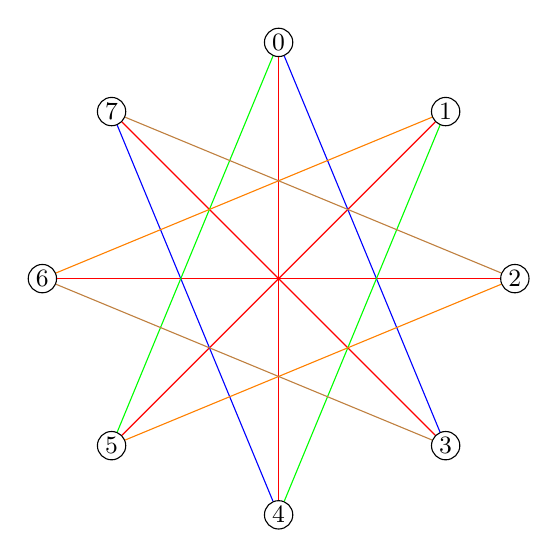
\begin{tikzpicture}[scale=3,
      every node/.style={circle, draw, fill=white, inner sep=1pt, font=\small}]
    
    % 1. Coloca os vértices uniformemente em círculo
    \foreach \i in {0,...,7} {
      \pgfmathsetmacro\angle{90-360*\i/8}
      \node (v\i) at (\angle:1) {\i};       % vértice v_i na posição angular correspondente
    }

    \draw [red] (v0)--(v4);
    \draw [red] (v1)--(v5);
    \draw [red] (v2)--(v6);
    \draw [red] (v3)--(v7);

    \draw [blue] (v0)--(v3);
    \draw [blue] (v7)--(v4);

    \draw [green] (v1)--(v4);
    \draw [green] (v0)--(v5);

    \draw [orange] (v1)--(v6);
    \draw [orange] (v2)--(v5);

    \draw [brown] (v3)--(v6);
    \draw [brown] (v2)--(v7);

    \end{tikzpicture}
  \end{center}

  Como a remoção de cada uma das partes deixa $G$ bipartido, podemos aplicar o Lema \ref{lem:odd-transversal} a $G$.
  Isso conclui a prova do Teorema. 
\end{proof}


%%%%%%%%%%%%%%%%%%%%%%%%%%%% APÊNDICES E ANEXOS %%%%%%%%%%%%%%%%%%%%%%%%%%%%%%%%

% Um apêndice é algum conteúdo adicional de sua autoria que faz parte e
% colabora com a ideia geral do texto mas que, por alguma razão, não precisa
% fazer parte da sequência do discurso; por exemplo, a demonstração de um
% teorema intermediário, as perguntas usadas em uma pesquisa qualitativa etc.
%
% Um anexo é um documento que não faz parte da tese (em geral, nem é de sua
% autoria) mas é relevante para o conteúdo; por exemplo, a especificação do
% padrão técnico ou a legislação que o trabalho discute, um artigo de jornal
% apresentando a percepção do público sobre o tema da tese etc.
%
% Os comandos appendix e annex reiniciam a numeração de capítulos e passam
% a numerá-los com letras. "annex" não faz parte de nenhuma classe padrão,
% foi criado para este modelo. Se o trabalho não tiver apêndices ou anexos,
% remova estas linhas.
%
% Diferentemente de \mainmatter, \backmatter etc., \appendix e \annex não
% forçam o início de uma nova página. Em geral isso não é importante, pois
% o comando seguinte costuma ser "\chapter", mas pode causar problemas com
% a formatação dos cabeçalhos. Assim, vamos forçar uma nova página antes
% de cada um deles.

%%%% Apêndices %%%%

\cleardoublepage

\pagestyle{appendix}

\appendix

% \addappheadtotoc acrescenta a palavra "Apêndice" ao sumário; se
% só há apêndices, sem anexos, provavelmente não é necessário.
% \addappheadtotoc

%%!TeX root=../tese.tex
%("dica" para o editor de texto: este arquivo é parte de um documento maior)
% para saber mais: https://tex.stackexchange.com/q/78101

\chapter{Perguntas frequentes sobre o modelo}

\begin{itemize}

\item \textbf{Não consigo decorar tantos comandos!}\\
Use a colinha que é distribuída juntamente com este modelo (\url{gitlab.com/ccsl-usp/modelo-latex/raw/main/pre-compilados/colinha.pdf?inline=false}).

\item \textbf{Estou tendo problemas com caracteres acentuados.}\\
Versões modernas de \LaTeX{} usam UTF-8, mas arquivos antigos podem usar outras codificações (como ISO-8859-1, também conhecido como latin1 ou Windows-1252). Nesses casos, use \textsf{\textbackslash{}usepackage[latin1]\{inputenc\}} no preâmbulo do documento. Você também pode representar os caracteres acentuados usando comandos \LaTeX{}: \textsf{\textbackslash\textquotesingle{}a} para á, \textsf{\textbackslash{}c\{c\}} para cedilha etc., independentemente da codificação usada no texto\footnote{Você pode consultar os comandos desse tipo mais comuns em \url{en.wikibooks.org/wiki/LaTeX/Special_Characters}. Observe que a dica sobre o pingo do i \emph{não} é mais válida atualmente; basta usar \textsf{\textbackslash\textquotesingle{}i}.}.

\item \textbf{É possível resumir o nome das seções/capítulos que aparece no topo das páginas e no sumário?}\\
Sim, usando a sintaxe \textsf{\textbackslash{}section[mini-titulo]\{titulo enorme\}}. Isso é especialmente útil nas legendas (\textit{captions}\index{Legendas}) das figuras e tabelas, que muitas vezes são demasiadamente longas para a lista de figuras/tabelas.

\item \textbf{Existe algum programa para gerenciar referências em formato bibtex?}\\
Sim, há vários. Uma opção bem comum é o JabRef; outra é usar Zotero\index{Zotero} ou Mendeley\index{Mendeley} e exportar os dados deles no formato .bib.

\item \textbf{Posso usar pacotes \LaTeX{} adicionais aos sugeridos?}\\
Com certeza! Você pode modificar os arquivos o quanto desejar, o modelo serve só como uma ajuda inicial para o seu trabalho.

\end{itemize}

\par

%%%% Anexos %%%%

\cleardoublepage

\pagestyle{appendix} % repete o anterior, caso você não use apêndices

\annex

% \addappheadtotoc acrescenta a palavra "Anexo" ao sumário; se
% só há anexos, sem apêndices, provavelmente não é necessário.
%\addappheadtotoc

%%!TeX root=../tese.tex
%("dica" para o editor de texto: este arquivo é parte de um documento maior)
% para saber mais: https://tex.stackexchange.com/q/78101

\chapter{As packages \pkg{imegoodies} e \pkg{imelooks}}
\label{ann:imegoodlooks}

Este modelo inclui as \textit{packages} \pkg{imegoodies} e \pkg{imelooks},
que você pode querer usar em outros documentos \LaTeX.

\pkg{imegoodies} inclui um grande número de \textit{packages} que são
comumente usadas e bastante úteis. Em geral, você pode incluí-la em seus
documentos sem que isso cause problemas de compatibilidade. Se, no
entanto, algo não funcionar, você pode editar o arquivo para eliminar
a \textit{package} responsável pelo problema se ela não for necessária.
\pkg{imegoodies} ainda inclui vários comentários explicativos sobre as
\textit{packages} carregadas.

\pkg{imelooks} também inclui um grande número de \textit{packages}, mas
estas são relacionadas mais explicitamente à aparência do documento
(fontes, cores, margens etc.). Você também pode utilizá-la em outros
documentos se quiser se aproximar da aparência deste modelo. \pkg{imelooks}
reconhece diversos parâmetros que ativam/desativam aspectos específicos:

\begin{itemize}
  \item \cmd{fonts} carrega as fontes deste modelo (libertinus e
        sourcecodepro), além de outros pequenos ajustes relacionados.
        Esta opção é sempre ativada por padrão; para desativá-la, use
        \cmd{nofonts}

  \item \cmd{spacing} utiliza os espaçamentos definidos neste modelo (margens,
        espaço entre parágrafos, indentação da primeira linha do parágrafo
        etc.). Esta opção é sempre ativada por padrão; para desativá-la, use
        \cmd{nospacing}

  \item \cmd{captions} e \cmd{footnotes} fazem respectivamente as legendas
        (das figuras e tabelas) e as notas de rodapé de acordo com este modelo.
        Estas opções são sempre ativadas por padrão; para desativá-las, use
        \cmd{nocaptions} e \cmd{nofootnotes}

  \item \cmd{autohttp} acrescenta o prefixo \cmd{http://} a URLs criadas
        com \ltxcmd{url} que não incluam o \textit{schema}. Esta opção é
        sempre ativada por padrão; para desativá-la, use \cmd{noautohttp}

  \item \cmd{hidelinks}, \cmd{borderlinks} e \cmd{colorlinks} definem a
        aparência dos hiperlinks. \cmd{hidelinks} faz os hiperlinks sem
        nenhuma formatação especial; \cmd{borderlinks} faz os hiperlinks
        serem envidos por um quadrado colorido (apenas na tela; o quadrado
        não é impresso); \cmd{colorlinks} faz o texto dos hiperlinks ser
        colorido. A opção \cmd{colorlinks} é sempre ativada por padrão

  \item \cmd{biblatex} carrega a \textit{package} \cmd{biblatex} e os
        estilos bibliográficos deste modelo. Esta opção é sempre ativada
        por padrão; para desativá-la, use \cmd{nobiblatex}
  \item \cmd{raggedbib} faz a bibliografia (com \cmd{biblatex}) ser
        formatada com alinhamento à esquerda ao invés de justificado.
        Esta opção é sempre ativada por padrão, exceto quando o estilo
        bibliográfico é \cmd{plainnat-ime} (usado nas teses); para
        desativá-la, use \cmd{noraggedbib}; para ativá-la incondicionalmente,
        use \cmd{raggedbib}
  \item \cmd{bibstyle=?} selectiona um estilo bibliográfico específico.
        O estilo padrão é \cmd{numeric}, exceto em pôsteres e apresentações
        (\cmd{beamer-ime}) e \textit{reports} (\cmd{plainnat-ime})

  \item \cmd{listings} carrega a \textit{package} \cmd{listings} e diversas
        configurações relacionadas usadas neste modelo. Esta opção é
        sempre ativada por padrão; para desativá-la, use \cmd{nolistings}

  \item \cmd{greeny}, \cmd{bluey}, \cmd{sandy} ativam esquemas de cores
        diferentes para pôsteres e apresentações (o padrão é \cmd{bluey})

  \item \cmd{beamer} \textbf{des}ativa algumas \textit{packages} que
        são incompatíveis com a classe \cmd{beamer} (note que as opções
        \cmd{slides} e \cmd{presentation}, discutidas abaixo, já fazem isso)

  \item \cmd{presentation} (ou \cmd{slides}) e \cmd{poster} ativam as
        opções relevantes para, respectivamente, apresentações com
        \cmd{beamer} ou pôsteres com \cmd{tcolorbox}

  \item \cmd{report} ativa as opções relevantes para documentos com
        capítulos (cabeçalhos das páginas, características do sumário etc.)

  \item \cmd{thesis} ativa a opção \cmd{report} e também define o que é
        necessário para a geração da capa das teses de acordo com este modelo

  \item \cmd{resumoabstract} define os comandos \cmd{resumo} e \cmd{abstract}
        de acordo com este modelo. Esta opção é ativada por padrão com
        \cmd{report}; para desativá-la, use \cmd{noresumoabstract}

  \item \cmd{brazilian} verifica se a língua portuguesa está ativa no
        documento e, em caso negativo, gera um erro. Esta opção é
        ativada por padrão com a opção \cmd{thesis}; para desativá-la,
        use \cmd{nobrazilian}
\end{itemize}

\par
%%!TeX root=../tese.tex
%("dica" para o editor de texto: este arquivo é parte de um documento maior)
% para saber mais: https://tex.stackexchange.com/q/78101

\chapter{Código-fonte e pseudocódigo}
\label{ap:pseudocode}

Com a \textit{package} \textsf{listings}, programas podem ser inseridos
diretamente no arquivo, como feito no caso do Programa~\ref{prog:java},
ou importados de um arquivo externo com o comando
\textsf{\textbackslash{}lstinputlisting}, como no caso
do Programa~\ref{prog:mdcinput}.

% O exemplo foi copiado da documentação de algorithmicx
\begin{program}
  \lstinputlisting[
    language=pseudocode,
    style=pseudocode,
    style=wider,
    functions={},
    specialidentifiers={},
  ]
  {conteudo/euclid.psc}

  \caption{Máximo divisor comum (arquivo importado).\label{prog:mdcinput}}
\end{program}

Trechos de código curtos (menores que uma página) podem ou não ser
incluídos como \textit{floats}; trechos longos necessariamente incluem
quebras de página e, portanto, não podem ser \textit{floats}. Com
\textit{floats}, a legenda e as linhas separadoras são colocadas pelo
comando \textsf{\textbackslash{}begin\{program\}}; sem eles, utilize o
ambiente \textsf{programruledcaption} (atenção para a colocação do
comando \textsf{\textbackslash{}label\{\}}, dentro da legenda), como
no Programa~\ref{prog:mdc}\footnote{\textsf{listings} oferece alguns
recursos próprios para a definição de \textit{floats} e legendas, mas
neste modelo não os utilizamos.}:

\begin{programruledcaption}{Máximo divisor comum (em português).\label{prog:mdc}}
  \begin{lstlisting}[
    language={[brazilian]pseudocode},
    style=pseudocode,
    style=wider,
    functions={},
    specialidentifiers={},
  ]
      funcao euclides(a, b) // O máximo divisor comum de \textbf{a} e \textbf{b}
          r := a $\bmod$ b
	  enquanto r != 0 // Atingimos a resposta se \textbf{r} é zero
              a := b
              b := r
              r := a $\bmod$ b
          fim
	  devolva b // O máximo divisor comum é \textbf{b}
      fim
  \end{lstlisting}
\end{programruledcaption}

Além do suporte às várias linguagens incluídas em \textsf{listings},
este modelo traz uma extensão para permitir o uso de pseudocódigo,
útil para a descrição de algoritmos em alto nível. Ela oferece
diversos recursos:

\begin{itemize}

    \item Comentários seguem o padrão de C++ (\lstinline{//} e
          \lstinline{/* ... */}), mas o delimitador é impresso
          como ``$\triangleright$''.

    \item ``:='', ``<>'', ``<='', ``>='' e ``!='' são substituídos
          pelo símbolo matemático adequado.

    \item É possível acrescentar palavras-chave além de ``if'', ``and''
          etc. com a opção ``\textsf{morekeywords=\{pchave1,\linebreak[0]{}pchave2\}}''
          (para um trecho de código específico) ou com o comando
          \textsf{\textbackslash{}lstset\{morekeywords=\linebreak[0]{}\{pchave1,pchave2\}\}}
          (como comando de configuração geral).

    \item É possível usar pequenos trechos de código, como nomes de variáveis,
          dentro de um parágrafo normal com \textsf{\textbackslash{}lstinline\{blah\}}.

    \item ``\$\dots\$'' ativa o modo matemático em qualquer lugar.

    \item Outros comandos \LaTeX{} funcionam apenas em comentários; fora, a
          linguagem simula alguns pré-definidos (\textsf{\textbackslash{}textit\{\}},
          \textsf{\textbackslash{}texttt\{\}} etc.).

    \item O comando \textsf{\textbackslash{}label} também funciona em
          comentários; a referência correspondente (\textsf{\textbackslash{}ref})
          indica o número da linha de código. Se quiser usá-lo numa linha sem
          comentários, use \lstinline{///}~\textsf{\textbackslash{}label\{blah\}};
          ``\lstinline{///}'' funciona como \lstinline{//}, permitindo
          a inserção de comandos \LaTeX{}, mas não imprime o delimitador
          (\ensuremath{\triangleright}).

    \item Para suspender a formatação automática, use \textsf{\textbackslash{}noparse\{blah\}}.

    \item Para forçar a formatação de um texto como função, identificador,
          palavra-chave ou comentário, use \textsf{\textbackslash{}func\{blah\}},
          \textsf{\textbackslash{}id\{blah\}}, \textsf{\textbackslash{}kw\{blah\}} ou
          \textsf{\textbackslash{}comment\{blah\}}.

    \item Palavras-chave dentro de comentários não são formatadas
          automaticamente; se necessário, use \textsf{\textbackslash{}func\{\}},
          \textsf{\textbackslash{}id\{\}} etc. ou comandos \LaTeX{} padrão.

    \item As palavras ``Program'', ``Procedure'' e ``Function'' têm formatação
          especial e fazem a palavra seguinte ser formatada como função.
          Funções em outros lugares \emph{não} são detectadas automaticamente;
          use \textsf{\textbackslash{}func\{\}}, a opção ``\textsf{functions=\{func1,func2\}}''
          ou o comando ``\textsf{\textbackslash{}lstset\{functions=\{func1,func2\}\}}''
          para que elas sejam detectadas.

    \item Além de funções, palavras-chave, strings, comentários e
          identificadores, há ``\textsf{specialidentifiers}''. Você pode
          usá-los com \textsf{\textbackslash{}specialid\{blah\}}, com a opção
          ``\textsf{specialidentifiers=\{id1,id2\}}'' ou com o comando
          ``\textsf{\textbackslash{}lstset\{specialidentifiers=\{id1,id2\}\}}''.

\end{itemize}



\par


%%%%%%%%%%%%%%% SEÇÕES FINAIS (BIBLIOGRAFIA E ÍNDICE REMISSIVO) %%%%%%%%%%%%%%%%

% O comando backmatter desabilita a numeração de capítulos.
\backmatter

\pagestyle{backmatter}

% Espaço adicional no sumário antes das referências / índice remissivo
\addtocontents{toc}{\vspace{2\baselineskip plus .5\baselineskip minus .5\baselineskip}}

% A bibliografia é obrigatória

\printbibliography[
  title=\refname\label{sec:bib}, % "Referências", recomendado pela ABNT
  %title=\bibname\label{sec:bib}, % "Bibliografia"
  heading=bibintoc, % Inclui a bibliografia no sumário
]

%\printindex % imprime o índice remissivo no documento (opcional)

\end{document}
